\documentclass[11pt]{article}

\usepackage[margin=1in]{geometry}
\usepackage{amsmath}
\usepackage{booktabs}
\usepackage{graphicx}
\usepackage{subcaption}
\usepackage{float}
\usepackage{microtype}

\graphicspath{{vae_outputs/}}

\title{Variational Autoencoders on Two-Moons Data and Conditional MNIST}
\author{Angel Rodriguez}
\date{\today}

\begin{document}
\maketitle

\begin{abstract}
This report studies variational autoencoders (VAEs) on a synthetic two-dimensional
two-moons distribution and on handwritten MNIST digits. The experiments vary both
the dimension of the latent space and the width/depth of the neural network.
Performance is evaluated using reconstruction and Kullback--Leibler (KL) losses,
but generated samples are treated as the primary qualitative criterion. On the
two-moons problem, a latent dimension of two is sufficient to represent the
distribution, and increasing the latent dimension does not improve the samples.
On conditional MNIST, the two-dimensional latent model produced the most
convincing samples in the visual comparison, even though larger latent spaces
achieved lower reconstruction losses. Changing network width and depth had a
smaller visual effect than changing the latent dimension; the deepest model was
only marginally better than the medium and shallow alternatives.
\end{abstract}

\section{Introduction}

Variational autoencoders combine an encoder, a probabilistic latent
representation, and a decoder. Unlike a conventional autoencoder, a VAE is
trained so that its latent representation remains close to a chosen prior,
usually a standard normal distribution. This makes it possible to generate new
samples by drawing a latent vector from the prior and passing it through the
decoder.

The goal of this assignment was to implement a VAE, first on an easy-to-visualize
two-dimensional distribution and then on a more interesting conditional image
generation problem. The experiments address two questions:
\begin{enumerate}
    \item How does the size of the latent space affect reconstruction, latent
    regularization, and generated samples?
    \item How much does network width and depth matter when the latent dimension
    is held fixed?
\end{enumerate}
The analysis emphasizes newly generated samples rather than relying only on
training or test error. This distinction is important because a model can
reconstruct held-out examples well without producing useful samples from its
prior.

\section{Model and objective}

\subsection{VAE formulation}

For an input $x$, the encoder produces a mean $\mu(x)$ and log variance
$\log \sigma^2(x)$. A latent sample is obtained with the reparameterization
trick:
\[
    z = \mu(x) + \sigma(x) \odot \epsilon,
    \qquad \epsilon \sim \mathcal{N}(0,I).
\]
The decoder maps $z$ to reconstruction logits. For a conditional model, the
class label is converted to a one-hot vector and concatenated to the encoder
input and decoder latent vector. Thus, the class label is available both when
encoding an image and when generating a new image.

The training objective is
\[
    \mathcal{L}
    =
    \mathcal{L}_{\mathrm{reconstruction}}
    +
    \beta D_{\mathrm{KL}}\left(q_\phi(z\mid x)\,\|\,p(z)\right),
\]
where
\[
    D_{\mathrm{KL}}
    =
    -\frac{1}{2}\sum_j
    \left(1+\log\sigma_j^2-\mu_j^2-\sigma_j^2\right).
\]
The two-moons experiments use mean-squared error for reconstruction and
$\beta_{\max}=0.25$. MNIST uses binary cross-entropy with logits and
$\beta_{\max}=1$. In both cases, $\beta$ is warmed up over the first half of
training. The reported reconstruction and KL values are separate components;
KL is a regularization term, not another reconstruction error.

\subsection{Implementation and data}

The implementation uses PyTorch and the Adam optimizer with learning rate
$10^{-3}$. The full experiments use 40 epochs and a fixed random seed of 42.
The two-moons data contain 4,000 noisy points, split into 70\% training,
15\% validation, and 15\% test data. The points are standardized using
statistics computed from the training split.

For MNIST, the conditional VAE receives flattened $28\times28$ grayscale
images and one of ten digit labels. The experiment uses 12,000 training
examples, 2,000 validation examples, and 2,000 held-out test examples.
The default latent-dimension architecture has hidden layers $(256,128)$.
Generated images are obtained by sampling $z\sim\mathcal{N}(0,I)$ and
conditioning the decoder on a requested digit label.

\section{Two-moons experiments}

\subsection{Latent dimension}

The first experiment keeps the hidden architecture fixed at $(64,64)$ and
compares latent dimensions 1, 2, 4, and 8. The generated samples are shown in
Figure~\ref{fig:moon-latent}. A one-dimensional latent space can produce a
rough approximation, but a two-dimensional latent space is sufficient to
capture the two curved components. Increasing the dimension beyond two does
not visibly improve the distribution and can make the generated points less
focused.

\begin{table}[H]
\centering
\caption{Two-moons latent-dimension results.}
\label{tab:moon-latent}
\begin{tabular}{lrrrr}
\toprule
Latent dimension & Parameters & Validation total & Test reconstruction & Test KL \\
\midrule
1 & 8,900 & 0.659 & 0.260 & 1.730 \\
2 & 9,094 & 0.680 & 0.222 & 1.907 \\
4 & 9,482 & 0.698 & 0.218 & 1.915 \\
8 & 10,258 & 0.706 & 0.230 & 1.875 \\
\bottomrule
\end{tabular}
\end{table}

The numerical results do not identify a single winner independently of the
samples. Latent dimension four has the lowest test reconstruction loss by a
small margin, while latent dimension two has a slightly better validation
total than dimensions four and eight. The visual result is more informative
for this low-dimensional task: two dimensions provide enough capacity without
introducing unnecessary degrees of freedom.

\begin{figure}[H]
\centering
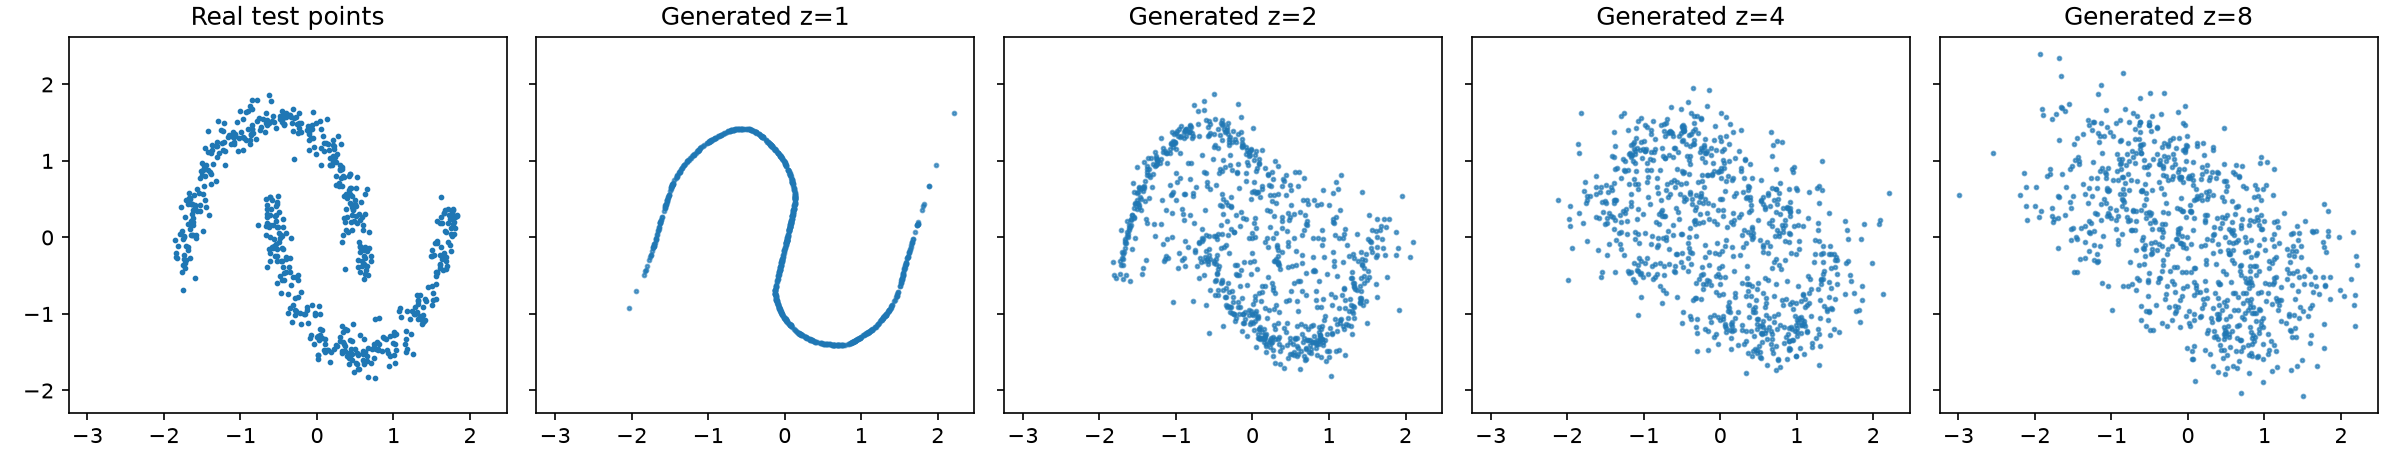
\includegraphics[width=0.82\textwidth]{moons_latent_samples.png}
\caption{Two-moons data and newly generated samples for different latent
dimensions. The samples should be judged by whether they form the two curved
components rather than by pointwise reconstruction alone.}
\label{fig:moon-latent}
\end{figure}

\subsection{Network width and depth}

The second two-moons experiment fixes the latent dimension at two and changes
the hidden layers. The shallow model uses one layer of width 32, the medium
model uses $(64,64)$, and the deep model uses $(128,128,128)$.

\begin{table}[H]
\centering
\caption{Two-moons architecture results with latent dimension two.}
\label{tab:moon-architecture}
\begin{tabular}{lrrrr}
\toprule
Architecture & Parameters & Validation total & Test reconstruction & Test KL \\
\midrule
Shallow-32 & 390 & 0.704 & 0.248 & 1.869 \\
Medium-64x2 & 9,094 & 0.680 & 0.222 & 1.907 \\
Deep-128x3 & 67,590 & 0.684 & 0.198 & 1.950 \\
\bottomrule
\end{tabular}
\end{table}

The deep model has the lowest test reconstruction loss, but it uses more than
seven times as many parameters as the medium model and more than 170 times as
many as the shallow model. The generated samples are all broadly successful,
so the visual improvement from adding depth and width is modest compared with
the computational cost. This supports the conclusion that the latent
dimension is the more important design choice for this distribution.

\begin{figure}[H]
\centering
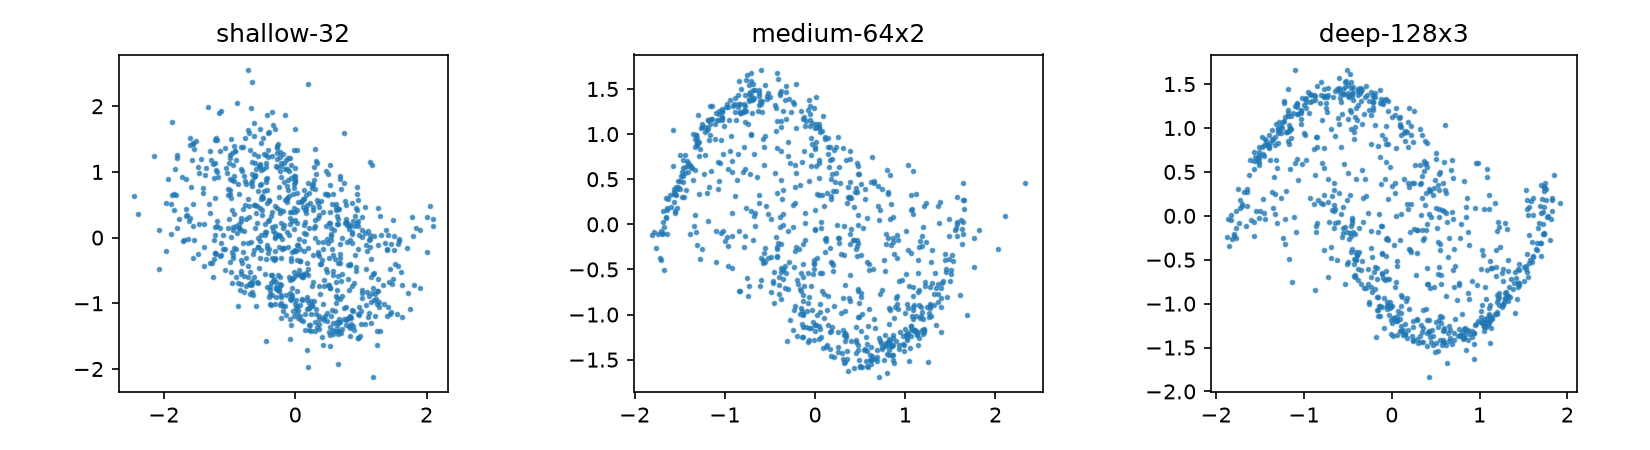
\includegraphics[width=0.82\textwidth]{moons_architecture_samples.png}
\caption{Generated two-moons samples for the shallow, medium, and deep
architectures.}
\label{fig:moon-architecture}
\end{figure}

\section{Conditional MNIST experiments}

\subsection{Latent dimension}

The MNIST latent-dimension experiment uses the same conditional architecture
for latent dimensions 2, 4, 8, 16, and 32. The generated grids request digits
0 through 9 from the decoder. The results are summarized in
Table~\ref{tab:mnist-latent}, and representative grids are shown in
Figure~\ref{fig:mnist-latent}.

\begin{table}[H]
\centering
\caption{Conditional MNIST latent-dimension results.}
\label{tab:mnist-latent}
\begin{tabular}{lrrrr}
\toprule
Latent dimension & Parameters & Validation total & Test reconstruction & Test KL \\
\midrule
2 & 473,108 & 134.937 & 130.714 & 4.772 \\
4 & 473,880 & 120.546 & 113.112 & 8.011 \\
8 & 475,424 & 109.528 & 95.071 & 14.085 \\
16 & 478,512 & 106.615 & 86.834 & 18.927 \\
32 & 484,688 & 106.386 & 86.899 & 19.009 \\
\bottomrule
\end{tabular}
\end{table}

The numerical reconstruction loss decreases substantially as the latent
dimension increases, with most of the improvement occurring by dimension 16.
The KL term increases because the larger latent representations carry more
information and therefore deviate more from the unit Gaussian prior. This is
not evidence that the larger models are incorrect: a lower KL term is not
always desirable, since excessive regularization can remove information needed
to represent the data.

The visual comparison gives a different result. In the generated grids, the
two-dimensional model produces the most recognizable and consistent
class-conditioned digits in this run. The larger latent models have lower
reconstruction losses, but their prior samples are visually less convincing
and progressively less reliable at following the requested digit. This
illustrates why generated samples must be examined in addition to
reconstruction metrics. It also suggests that a larger latent space can make
the posterior represent training examples more accurately without making the
prior-to-decoder path easier to sample from after finite training.

\begin{figure}[H]
\centering
\begin{subfigure}{0.48\textwidth}
    \centering
    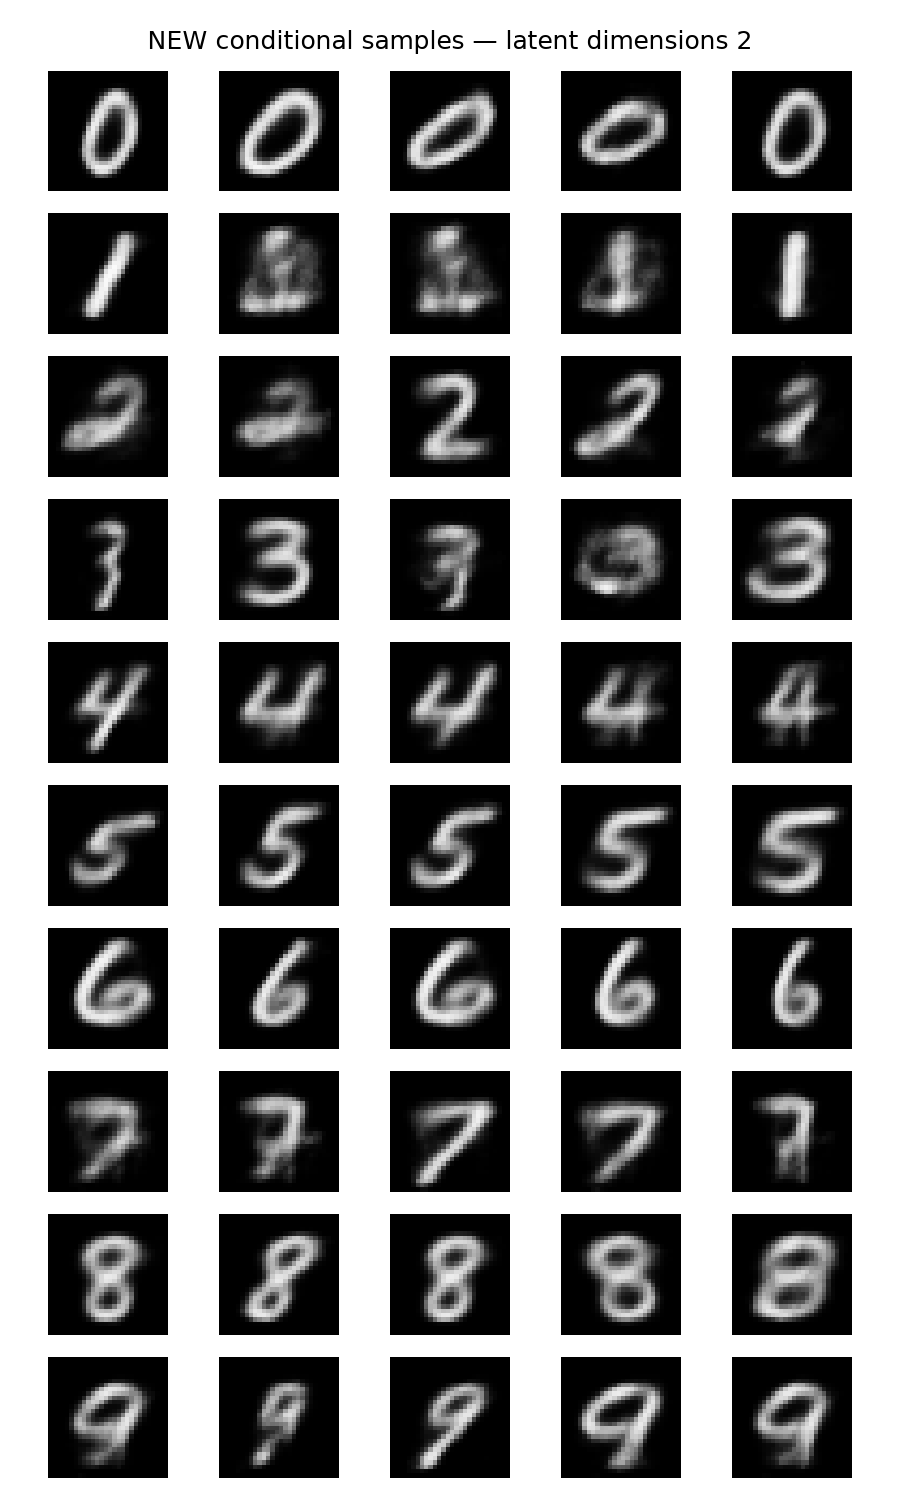
\includegraphics[width=\textwidth]{mnist_generated_z2.png}
    \caption{$z=2$}
\end{subfigure}
\begin{subfigure}{0.48\textwidth}
    \centering
    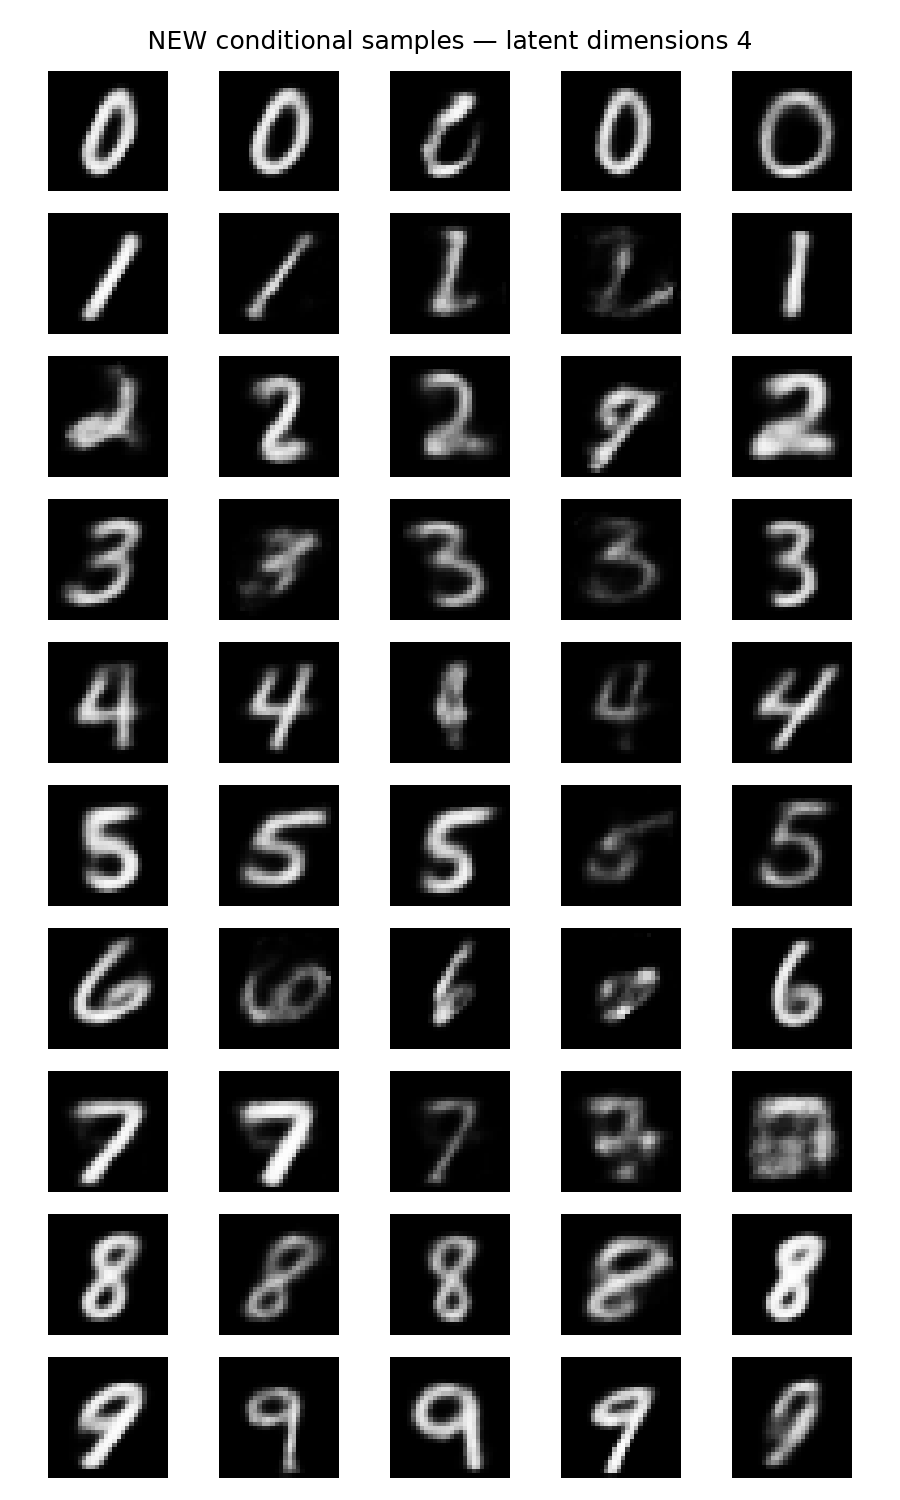
\includegraphics[width=\textwidth]{mnist_generated_z4.png}
    \caption{$z=4$}
\end{subfigure}

\begin{subfigure}{0.48\textwidth}
    \centering
    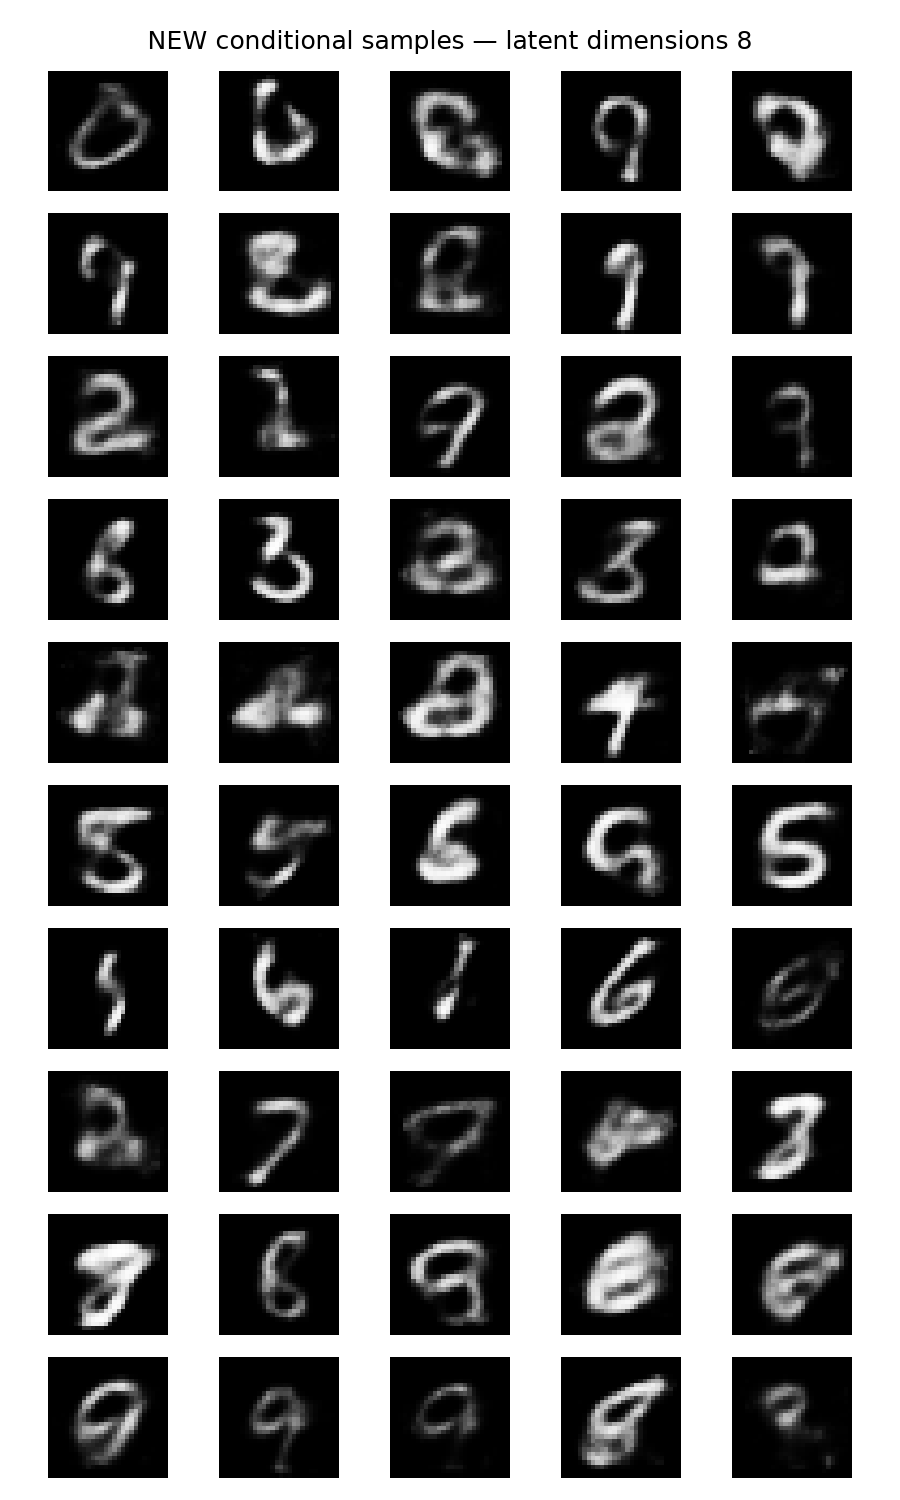
\includegraphics[width=\textwidth]{mnist_generated_z8.png}
    \caption{$z=8$}
\end{subfigure}
\begin{subfigure}{0.48\textwidth}
    \centering
    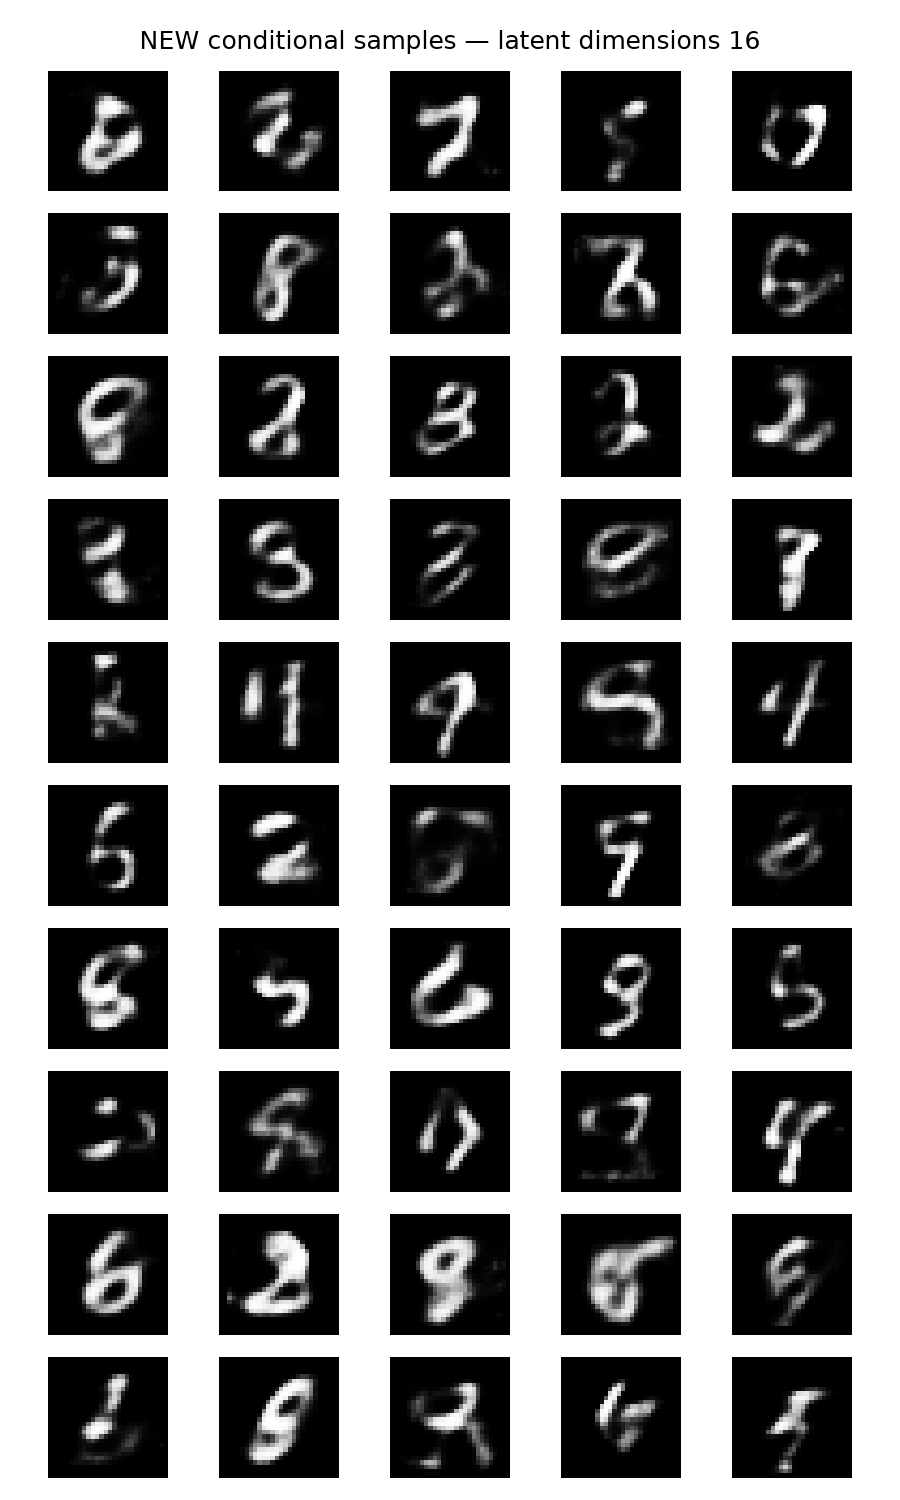
\includegraphics[width=\textwidth]{mnist_generated_z16.png}
    \caption{$z=16$}
\end{subfigure}

\begin{subfigure}{0.48\textwidth}
    \centering
    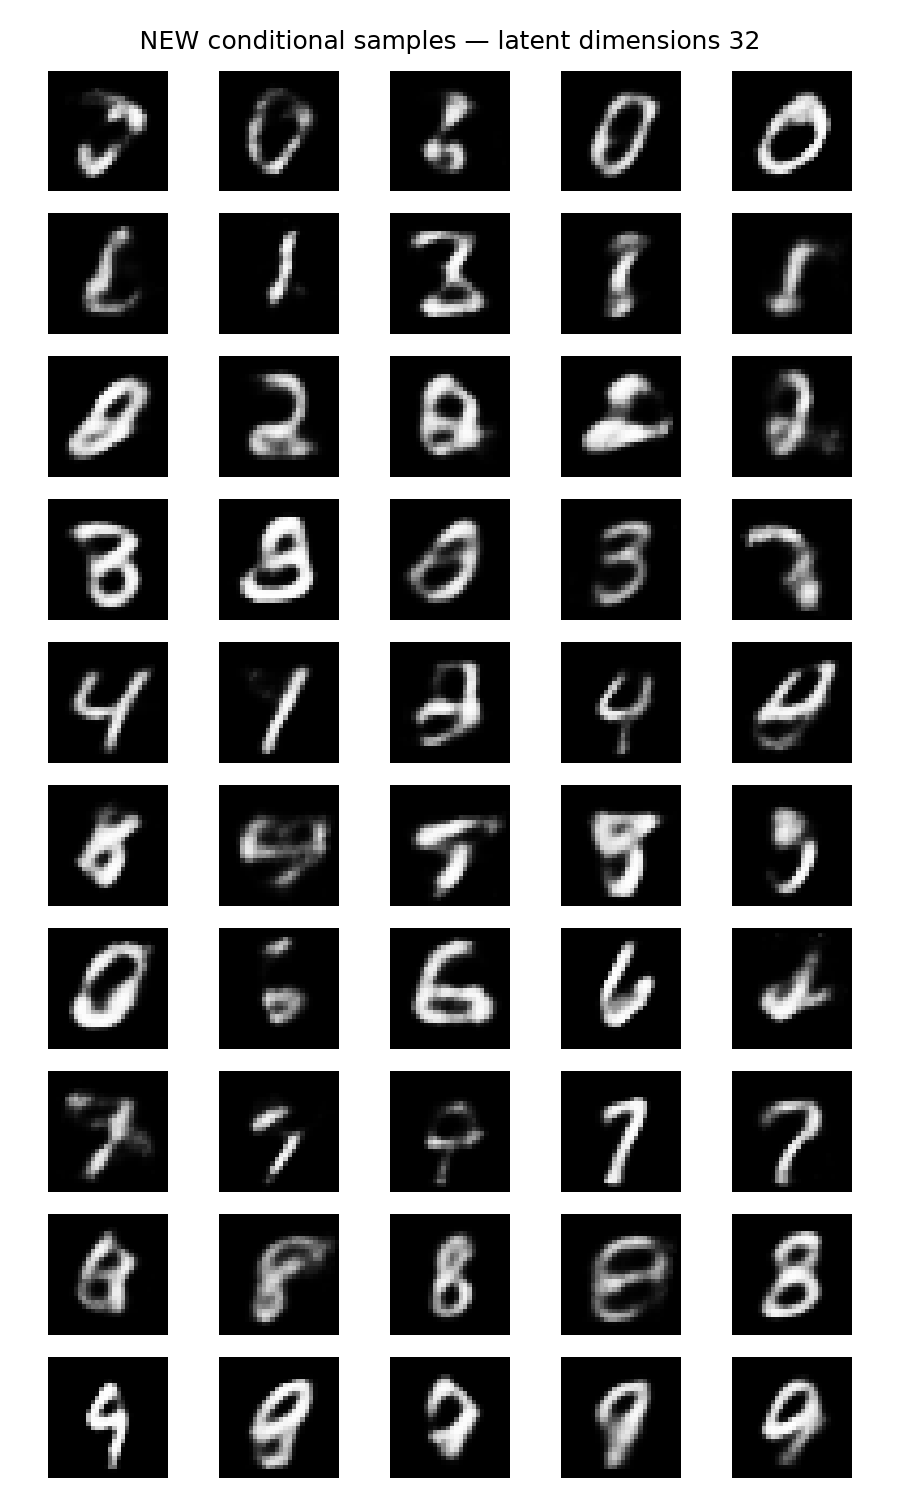
\includegraphics[width=\textwidth]{mnist_generated_z32.png}
    \caption{$z=32$}
\end{subfigure}
\caption{New conditional MNIST samples for each latent dimension. Each row
requests one digit class, rather than reconstructing a particular test image.}
\label{fig:mnist-latent}
\end{figure}

\subsection{Network architecture}

The architecture experiment fixes the latent dimension at two and compares
three conditional networks. The shallow, medium, and deep models use hidden
layers $(64)$, $(256,128)$, and $(256,128,64)$, respectively.

\begin{table}[H]
\centering
\caption{Conditional MNIST architecture results with latent dimension two.}
\label{tab:mnist-architecture}
\begin{tabular}{lrrrr}
\toprule
Architecture & Parameters & Validation total & Test reconstruction & Test KL \\
\midrule
Shallow-64 & 102,932 & 143.882 & 139.628 & 3.963 \\
Medium-256x128 & 473,108 & 134.937 & 130.714 & 4.772 \\
Deep-256x128x64 & 488,596 & 134.004 & 130.245 & 4.559 \\
\bottomrule
\end{tabular}
\end{table}

The deep model has the best reported validation total and the lowest test
reconstruction error, but its advantage over the medium model is small. The
generated images also look broadly similar across the three architectures.
The shallow network has fewer parameters and performs worse numerically, but
the medium and deep models are close in both sample quality and metrics. Thus,
for this experiment, increasing network depth and width has less visible
impact than changing the latent dimension.

\begin{figure}[H]
\centering
\begin{subfigure}{0.32\textwidth}
    \centering
    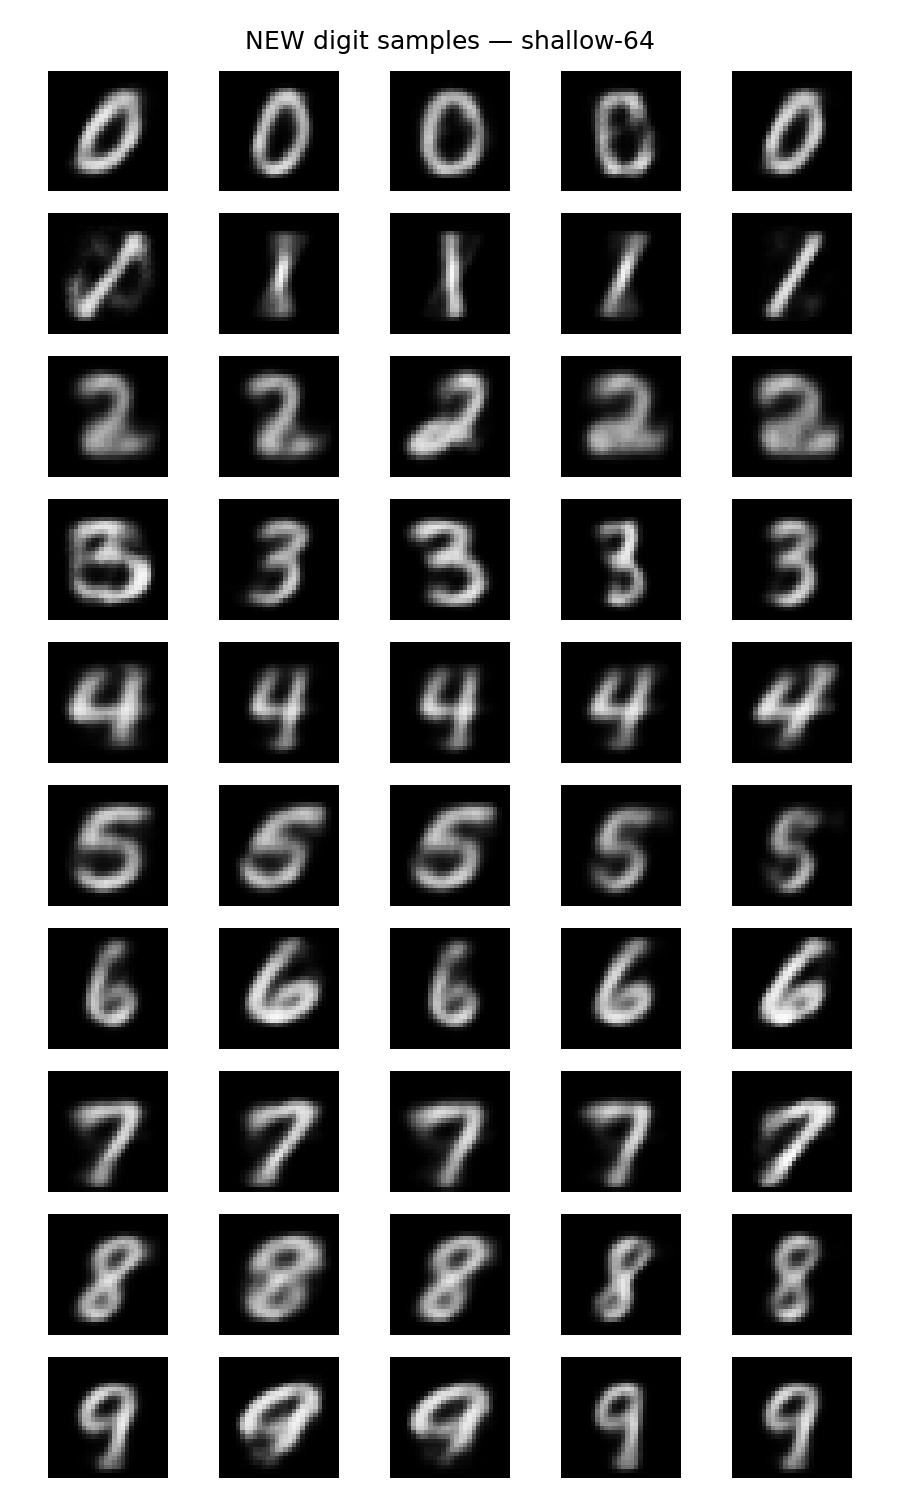
\includegraphics[width=\textwidth]{mnist_shallow-64.png}
    \caption{Shallow}
\end{subfigure}
\begin{subfigure}{0.32\textwidth}
    \centering
    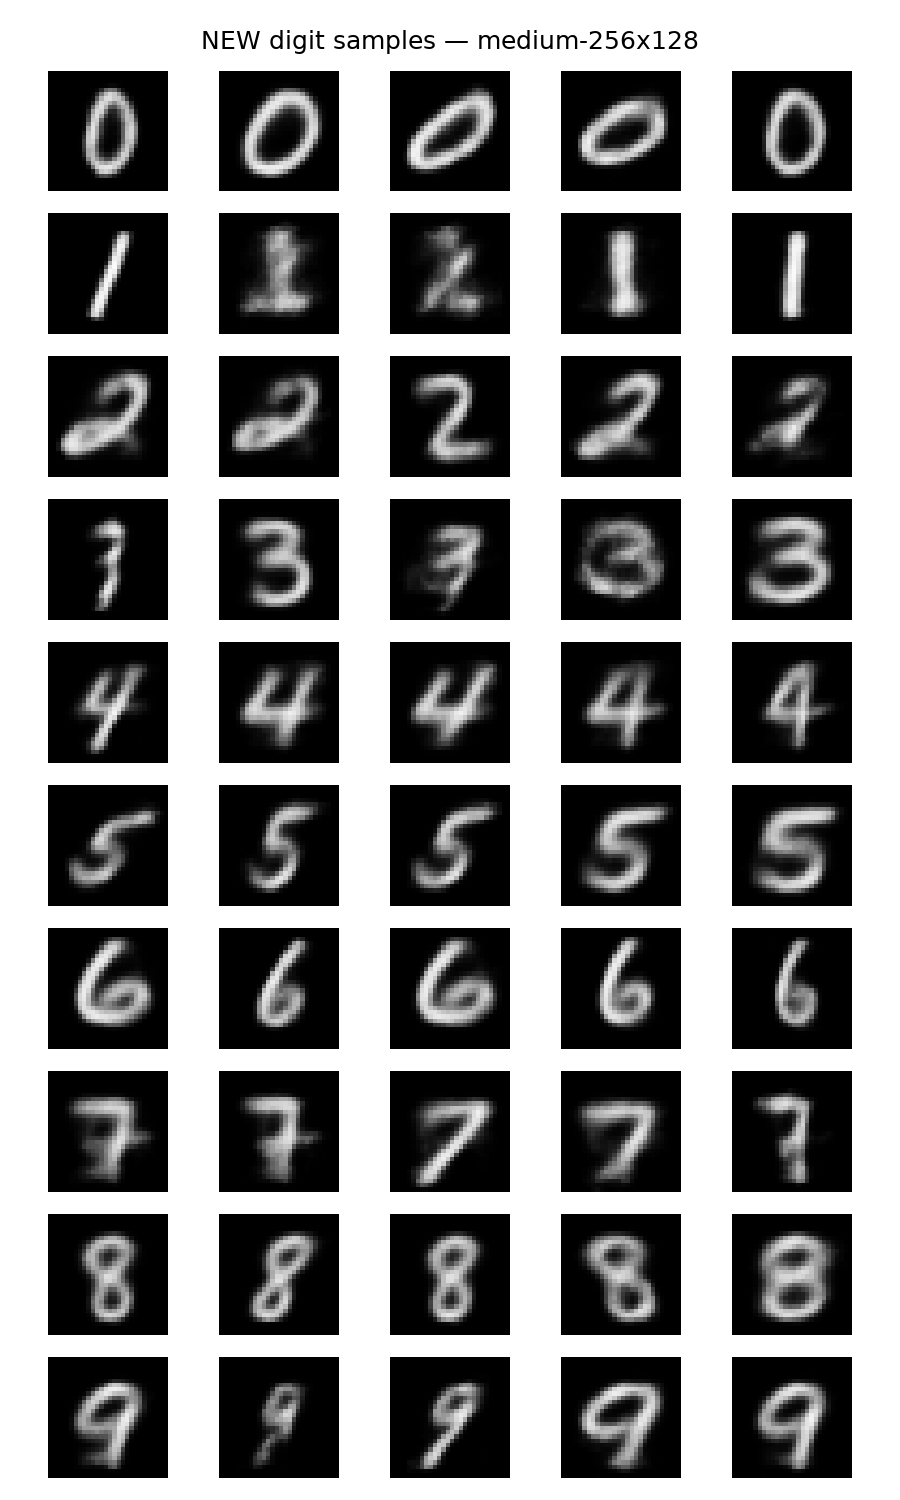
\includegraphics[width=\textwidth]{mnist_medium-256x128.png}
    \caption{Medium}
\end{subfigure}
\begin{subfigure}{0.32\textwidth}
    \centering
    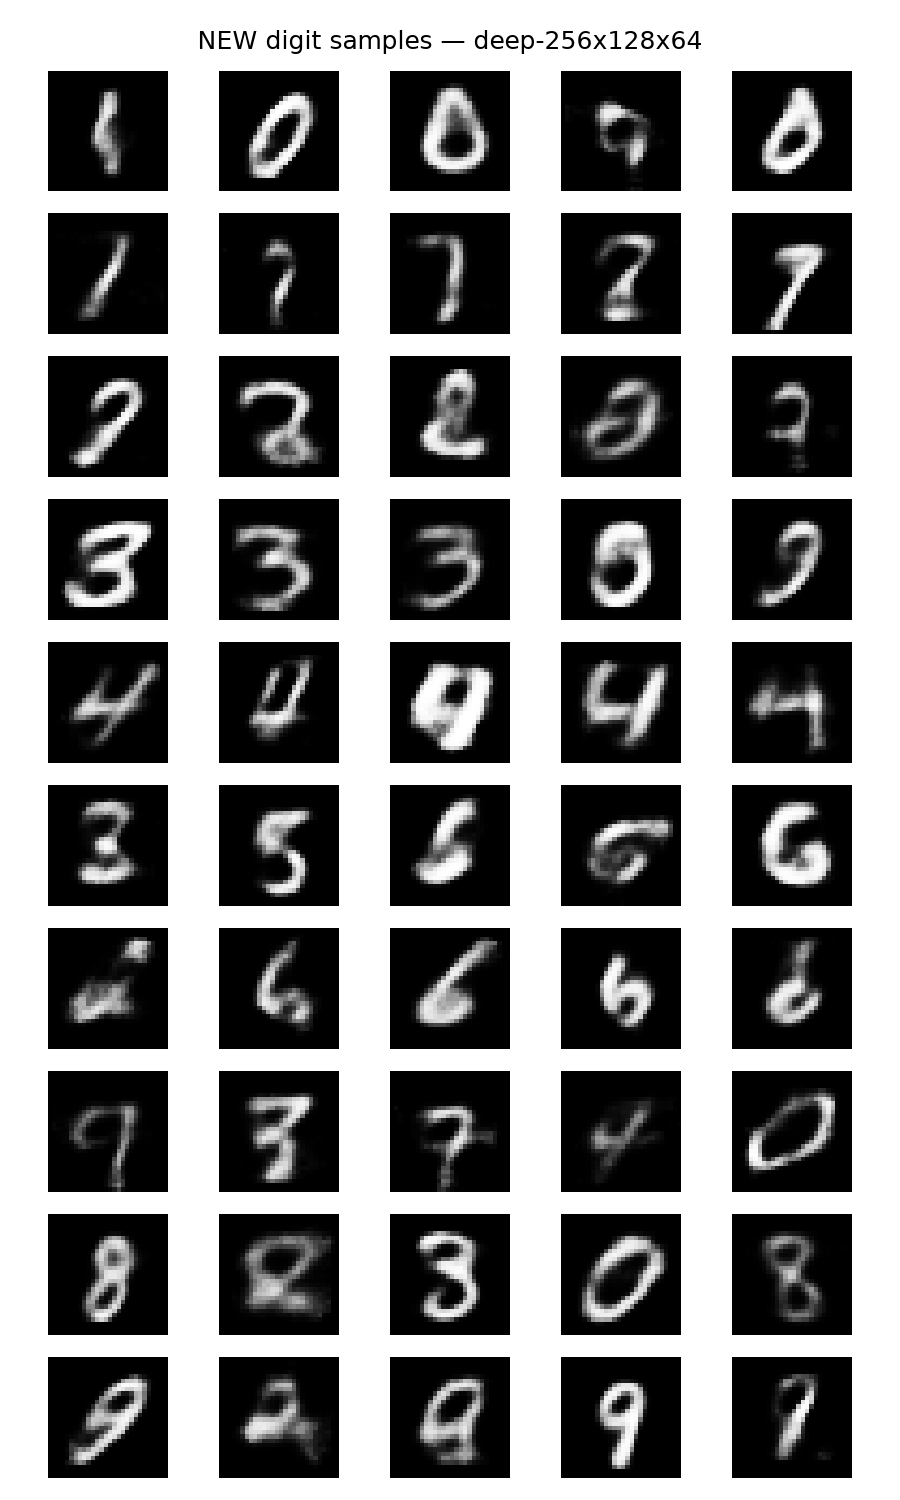
\includegraphics[width=\textwidth]{mnist_deep-256x128x64.png}
    \caption{Deep}
\end{subfigure}
\caption{New conditional MNIST samples for the architecture comparison.}
\label{fig:mnist-architecture}
\end{figure}

\subsection{Reconstructions versus new samples}

The final visualization separates three different tasks: reproducing held-out
images, generating new images from the prior, and obeying the requested
condition. Reconstructions pass test images through the encoder and decoder,
whereas new samples draw random latent vectors and provide only a digit label
to the decoder. The latter is the more demanding generative test.

\begin{figure}[H]
\centering
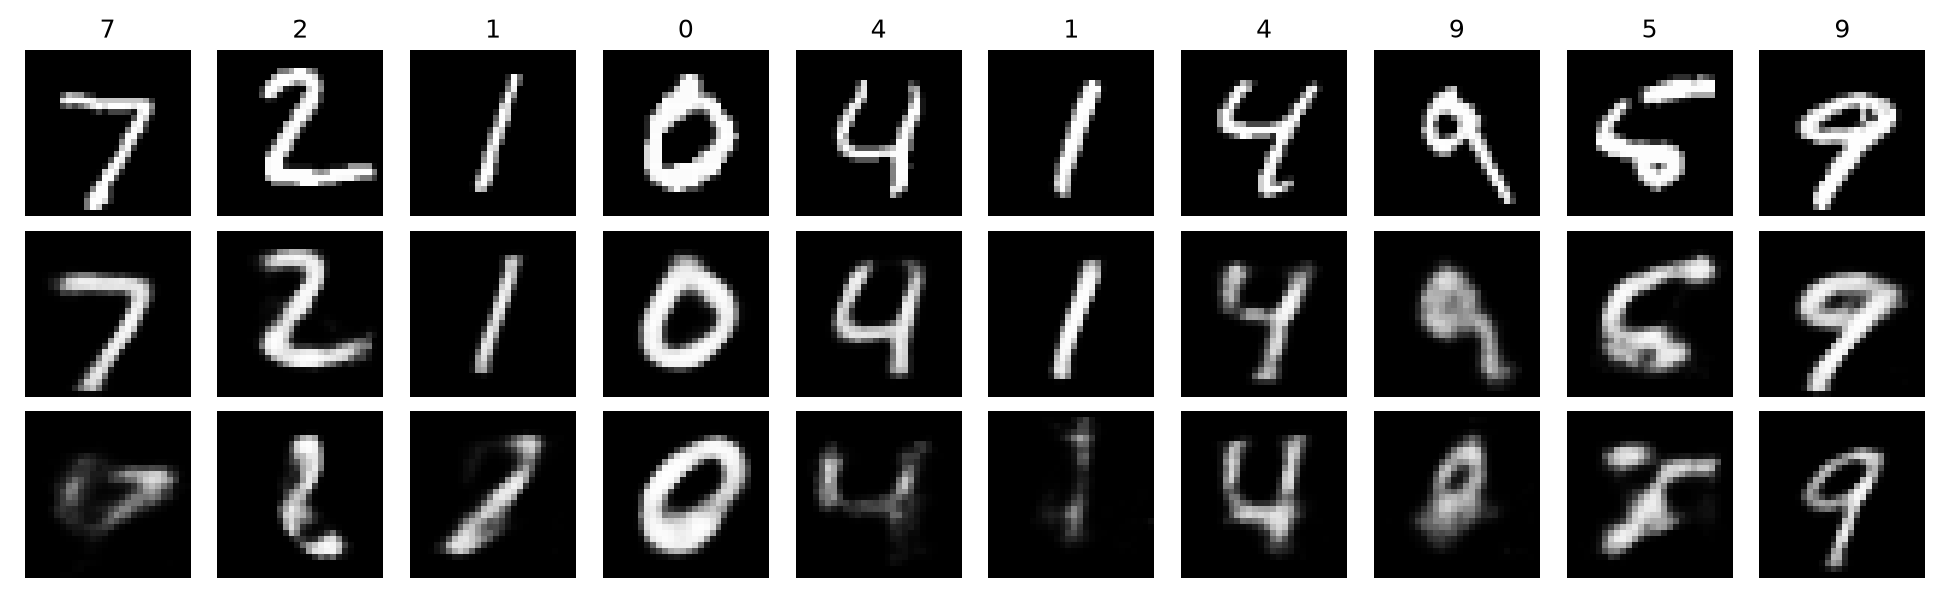
\includegraphics[width=\textwidth]{mnist_real_vs_reconstructed_vs_new.png}
\caption{Real test examples, their reconstructions, and newly generated
conditional samples. Column titles identify the requested digit.}
\label{fig:mnist-final}
\end{figure}

\section{Discussion}

Several conclusions emerge from the experiments.

\paragraph{Latent size is not simply a capacity knob.}
Increasing the latent dimension reduced MNIST reconstruction error, but the
visual quality of prior samples did not improve in the same way. The decoder
is trained primarily on latent vectors produced by the encoder. Sampling from
the prior requires the aggregate encoded distribution to align sufficiently
with that prior. A larger latent space can therefore improve reconstruction
while making prior sampling harder under the same training budget.

\paragraph{KL should be interpreted jointly with reconstruction.}
The KL term measures the distance between the encoder's approximate posterior
and the standard normal prior. A small KL can indicate strong regularization,
but it can also mean that the latent code carries little information. A large
KL can accompany better reconstructions because the model is using the latent
variables more actively. The relevant objective is the weighted sum, together
with the quality and diversity of generated samples.

\paragraph{Architecture has diminishing returns.}
For both datasets, larger networks reduce reconstruction error to some degree.
However, the visual difference between medium and deep networks is small,
especially on MNIST with a two-dimensional latent space. The additional
parameters are not automatically converted into better generative behavior.
This result is consistent with the idea that the bottleneck and prior
regularization constrain the model more strongly than the decoder's extra
capacity in these experiments.

\paragraph{Evaluation should include generation.}
The two-moons plots make distributional errors immediately visible, while the
MNIST grids reveal whether the requested class is preserved. These checks
would be missed by reporting only a reconstruction loss. In particular, the
MNIST latent-dimension experiment demonstrates that the numerically best
reconstruction model is not necessarily the visually best model for new
conditional samples.

\section{Limitations and future work}

The experiments use one random seed, a subset of MNIST, and a fixed training
schedule. The full MNIST runs use 40 epochs, so the apparent degradation of
larger latent spaces could partly reflect optimization time or the chosen
KL warm-up schedule rather than an inherent limitation of those dimensions.
The visual ranking is also based on a finite number of generated images and
human judgment. A more complete study would repeat each configuration across
several seeds, use a larger training set, tune the warm-up schedule, and
evaluate conditional sample quality with an automated classifier or a
class-conditional likelihood metric. It would also be useful to compare
latent dimensions and architectures using the same selected validation
criterion before reporting the held-out test results.

\section{Conclusion}

The VAE successfully learned the two-moons distribution and generated
class-conditioned MNIST digits. On the two-moons problem, a latent dimension
of two was sufficient; larger latent spaces did not provide a meaningful
visual benefit. On MNIST, larger latent spaces produced lower reconstruction
losses, but the two-dimensional model produced the best-looking new
conditional samples in the visual comparison. With latent dimension fixed at
two, the deep architecture was numerically and visually only slightly better
than the medium model, while the shallow model used far fewer parameters but
lost some performance. Overall, these results support selecting a VAE based
on both reconstruction/regularization metrics and the quality of samples
drawn from the latent prior.

\end{document}
